\documentclass[twoside]{book}

% Packages required by doxygen
\usepackage{calc}
\usepackage{doxygen}
\usepackage{graphicx}
\usepackage[utf8]{inputenc}
\usepackage{makeidx}
\usepackage{multicol}
\usepackage{multirow}
\usepackage{textcomp}
\usepackage[table]{xcolor}

% Font selection
\usepackage[T1]{fontenc}
\usepackage{mathptmx}
\usepackage[scaled=.90]{helvet}
\usepackage{courier}
\usepackage{amssymb}
\usepackage{sectsty}
\renewcommand{\familydefault}{\sfdefault}
\allsectionsfont{%
  \fontseries{bc}\selectfont%
  \color{darkgray}%
}
\renewcommand{\DoxyLabelFont}{%
  \fontseries{bc}\selectfont%
  \color{darkgray}%
}

% Page & text layout
\usepackage{geometry}
\geometry{%
  a4paper,%
  top=2.5cm,%
  bottom=2.5cm,%
  left=2.5cm,%
  right=2.5cm%
}
\tolerance=750
\hfuzz=15pt
\hbadness=750
\setlength{\emergencystretch}{15pt}
\setlength{\parindent}{0cm}
\setlength{\parskip}{0.2cm}
\makeatletter
\renewcommand{\paragraph}{%
  \@startsection{paragraph}{4}{0ex}{-1.0ex}{1.0ex}{%
    \normalfont\normalsize\bfseries\SS@parafont%
  }%
}
\renewcommand{\subparagraph}{%
  \@startsection{subparagraph}{5}{0ex}{-1.0ex}{1.0ex}{%
    \normalfont\normalsize\bfseries\SS@subparafont%
  }%
}
\makeatother

% Headers & footers
\usepackage{fancyhdr}
\pagestyle{fancyplain}
\fancyhead[LE]{\fancyplain{}{\bfseries\thepage}}
\fancyhead[CE]{\fancyplain{}{}}
\fancyhead[RE]{\fancyplain{}{\bfseries\leftmark}}
\fancyhead[LO]{\fancyplain{}{\bfseries\rightmark}}
\fancyhead[CO]{\fancyplain{}{}}
\fancyhead[RO]{\fancyplain{}{\bfseries\thepage}}
\fancyfoot[LE]{\fancyplain{}{}}
\fancyfoot[CE]{\fancyplain{}{}}
\fancyfoot[RE]{\fancyplain{}{\bfseries\scriptsize Generated on Tue Feb 13 2018 10\-:43\-:31 for Tibero Message Protocol by Doxygen }}
\fancyfoot[LO]{\fancyplain{}{\bfseries\scriptsize Generated on Tue Feb 13 2018 10\-:43\-:31 for Tibero Message Protocol by Doxygen }}
\fancyfoot[CO]{\fancyplain{}{}}
\fancyfoot[RO]{\fancyplain{}{}}
\renewcommand{\footrulewidth}{0.4pt}
\renewcommand{\chaptermark}[1]{%
  \markboth{#1}{}%
}
\renewcommand{\sectionmark}[1]{%
  \markright{\thesection\ #1}%
}

% Indices & bibliography
\usepackage{natbib}
\usepackage[titles]{tocloft}
\setcounter{tocdepth}{3}
\setcounter{secnumdepth}{5}
\makeindex

% Hyperlinks (required, but should be loaded last)
\usepackage{ifpdf}
\ifpdf
  \usepackage[pdftex,pagebackref=true]{hyperref}
\else
  \usepackage[ps2pdf,pagebackref=true]{hyperref}
\fi
\hypersetup{%
  colorlinks=true,%
  linkcolor=blue,%
  citecolor=blue,%
  unicode%
}

% Custom commands
\newcommand{\clearemptydoublepage}{%
  \newpage{\pagestyle{empty}\cleardoublepage}%
}


%===== C O N T E N T S =====

\begin{document}

% Titlepage & ToC
\hypersetup{pageanchor=false}
\pagenumbering{roman}
\begin{titlepage}
\vspace*{7cm}
\begin{center}%
{\Large Tibero Message Protocol }\\
\vspace*{1cm}
{\large Generated by Doxygen 1.8.6}\\
\vspace*{0.5cm}
{\small Tue Feb 13 2018 10:43:31}\\
\end{center}
\end{titlepage}
\clearemptydoublepage
\tableofcontents
\clearemptydoublepage
\pagenumbering{arabic}
\hypersetup{pageanchor=true}

%--- Begin generated contents ---
\chapter{Hierarchical Index}
\section{Class Hierarchy}
This inheritance list is sorted roughly, but not completely, alphabetically\-:\begin{DoxyCompactList}
\item \contentsline{section}{Partial\-Header}{\pageref{structPartialHeader}}{}
\item \contentsline{section}{Pipe}{\pageref{classPipe}}{}
\item \contentsline{section}{Raw\-Sendable}{\pageref{structRawSendable}}{}
\item \contentsline{section}{Receivable}{\pageref{classReceivable}}{}
\item \contentsline{section}{Serializable$<$ Derived\-Serializable $>$}{\pageref{classSerializable}}{}
\item \contentsline{section}{Serializable$<$ Derived\-Sendable $>$}{\pageref{classSerializable}}{}
\begin{DoxyCompactList}
\item \contentsline{section}{Sendable$<$ Derived\-Sendable $>$}{\pageref{classSendable}}{}
\end{DoxyCompactList}
\item \contentsline{section}{T\-C\-P\-Header}{\pageref{structTCPHeader}}{}
\end{DoxyCompactList}

\chapter{Class Index}
\section{Class List}
Here are the classes, structs, unions and interfaces with brief descriptions\-:\begin{DoxyCompactList}
\item\contentsline{section}{\hyperlink{structPartialHeader}{Partial\-Header} }{\pageref{structPartialHeader}}{}
\item\contentsline{section}{\hyperlink{classPipe}{Pipe} }{\pageref{classPipe}}{}
\item\contentsline{section}{\hyperlink{structRawSendable}{Raw\-Sendable} }{\pageref{structRawSendable}}{}
\item\contentsline{section}{\hyperlink{classReceivable}{Receivable} }{\pageref{classReceivable}}{}
\item\contentsline{section}{\hyperlink{classSendable}{Sendable$<$ Derived\-Sendable $>$} }{\pageref{classSendable}}{}
\item\contentsline{section}{\hyperlink{classSerializable}{Serializable$<$ Derived\-Serializable $>$} }{\pageref{classSerializable}}{}
\item\contentsline{section}{\hyperlink{structTCPHeader}{T\-C\-P\-Header} }{\pageref{structTCPHeader}}{}
\end{DoxyCompactList}

\chapter{File Index}
\section{File List}
Here is a list of all documented files with brief descriptions\-:\begin{DoxyCompactList}
\item\contentsline{section}{/home/hspark/\-Dev\-Works/\-H-\/\-Tmax/cpp\-Tests/\-Message\-Protocol/\-T\-C\-P/{\bfseries Pipe.\-h} }{\pageref{Pipe_8h}}{}
\item\contentsline{section}{/home/hspark/\-Dev\-Works/\-H-\/\-Tmax/cpp\-Tests/\-Message\-Protocol/\-T\-C\-P/{\bfseries Receivable.\-h} }{\pageref{Receivable_8h}}{}
\item\contentsline{section}{/home/hspark/\-Dev\-Works/\-H-\/\-Tmax/cpp\-Tests/\-Message\-Protocol/\-T\-C\-P/\hyperlink{Sendable_8h}{Sendable.\-h} \\*\hyperlink{classSendable}{Sendable} header file for T\-C\-P (Tibero Communication Protocol) }{\pageref{Sendable_8h}}{}
\item\contentsline{section}{/home/hspark/\-Dev\-Works/\-H-\/\-Tmax/cpp\-Tests/\-Message\-Protocol/\-T\-C\-P/\hyperlink{Serializable_8h}{Serializable.\-h} \\*\hyperlink{classSerializable}{Serializable} header file }{\pageref{Serializable_8h}}{}
\item\contentsline{section}{/home/hspark/\-Dev\-Works/\-H-\/\-Tmax/cpp\-Tests/\-Message\-Protocol/\-T\-C\-P/{\bfseries T\-C\-P.\-h} }{\pageref{TCP_8h}}{}
\item\contentsline{section}{/home/hspark/\-Dev\-Works/\-H-\/\-Tmax/cpp\-Tests/\-Message\-Protocol/\-T\-C\-P/{\bfseries T\-C\-P\-\_\-\-T\-Y\-P\-E\-\_\-\-L\-I\-S\-T.\-h} }{\pageref{TCP__TYPE__LIST_8h}}{}
\end{DoxyCompactList}

\chapter{Class Documentation}
\hypertarget{structPartialHeader}{\section{Partial\-Header Struct Reference}
\label{structPartialHeader}\index{Partial\-Header@{Partial\-Header}}
}
\subsection*{Public Attributes}
\begin{DoxyCompactItemize}
\item 
\hypertarget{structPartialHeader_a4b574e6aefd1eafc6f07be34787d5bd1}{long int {\bfseries I\-D}}\label{structPartialHeader_a4b574e6aefd1eafc6f07be34787d5bd1}

\item 
\hypertarget{structPartialHeader_a90cad17b14ba56d0ad33d5f34f548efe}{int {\bfseries sequence}}\label{structPartialHeader_a90cad17b14ba56d0ad33d5f34f548efe}

\item 
\hypertarget{structPartialHeader_acf3c2b2bb3e7a05992c6e9a54892df89}{int {\bfseries total\-Count}}\label{structPartialHeader_acf3c2b2bb3e7a05992c6e9a54892df89}

\end{DoxyCompactItemize}


The documentation for this struct was generated from the following file\-:\begin{DoxyCompactItemize}
\item 
/home/hspark/\-Dev\-Works/\-H-\/\-Tmax/cpp\-Tests/\-Message\-Protocol/\-T\-C\-P/T\-C\-P.\-h\end{DoxyCompactItemize}

\hypertarget{classPipe}{\section{Pipe Class Reference}
\label{classPipe}\index{Pipe@{Pipe}}
}
\subsection*{Public Member Functions}
\begin{DoxyCompactItemize}
\item 
\hypertarget{classPipe_abf05b8e0b2df21a45ed48d2aaf80370b}{int {\bfseries get\-Read\-Fd} ()}\label{classPipe_abf05b8e0b2df21a45ed48d2aaf80370b}

\item 
\hypertarget{classPipe_a7bd26dd1f35fc5584199a643b41a4799}{int {\bfseries get\-Write\-Fd} ()}\label{classPipe_a7bd26dd1f35fc5584199a643b41a4799}

\end{DoxyCompactItemize}


The documentation for this class was generated from the following file\-:\begin{DoxyCompactItemize}
\item 
/home/hspark/\-Dev\-Works/\-H-\/\-Tmax/cpp\-Tests/\-Message\-Protocol/\-T\-C\-P/Pipe.\-h\end{DoxyCompactItemize}

\hypertarget{structRawSendable}{\section{Raw\-Sendable Struct Reference}
\label{structRawSendable}\index{Raw\-Sendable@{Raw\-Sendable}}
}
\subsection*{Public Attributes}
\begin{DoxyCompactItemize}
\item 
\hypertarget{structRawSendable_ac8414dac88d017ad03f0d8f37cc99375}{int {\bfseries sendable\-I\-D}}\label{structRawSendable_ac8414dac88d017ad03f0d8f37cc99375}

\item 
\hypertarget{structRawSendable_ae1daa08239b08632a5ca6a7b626e9265}{int {\bfseries size}}\label{structRawSendable_ae1daa08239b08632a5ca6a7b626e9265}

\item 
\hypertarget{structRawSendable_ac607e993b6535e28ddeb2fbe498d0944}{byte $\ast$ {\bfseries serialized\-Payload}}\label{structRawSendable_ac607e993b6535e28ddeb2fbe498d0944}

\end{DoxyCompactItemize}


The documentation for this struct was generated from the following file\-:\begin{DoxyCompactItemize}
\item 
/home/hspark/\-Dev\-Works/\-H-\/\-Tmax/cpp\-Tests/\-Message\-Protocol/\-T\-C\-P/T\-C\-P.\-h\end{DoxyCompactItemize}

\hypertarget{classReceivable}{\section{Receivable Class Reference}
\label{classReceivable}\index{Receivable@{Receivable}}
}
\subsection*{Public Member Functions}
\begin{DoxyCompactItemize}
\item 
\hypertarget{classReceivable_a39a29183fdbf007225f4f9545856b658}{void {\bfseries tb\-\_\-recv} ()}\label{classReceivable_a39a29183fdbf007225f4f9545856b658}

\item 
\hypertarget{classReceivable_a18e6aff1e81b206d7040a220043dcbc4}{\hyperlink{structRawSendable}{Raw\-Sendable} $\ast$ {\bfseries get\-Raw\-Sendable} ()}\label{classReceivable_a18e6aff1e81b206d7040a220043dcbc4}

\item 
\hypertarget{classReceivable_aa164a5ac8424f8f10508192507992ddf}{int {\bfseries get\-Reading\-End} ()}\label{classReceivable_aa164a5ac8424f8f10508192507992ddf}

\item 
\hypertarget{classReceivable_a125e09e854697011e6ef081dcf8c2392}{int {\bfseries get\-Writing\-End} ()}\label{classReceivable_a125e09e854697011e6ef081dcf8c2392}

\end{DoxyCompactItemize}


The documentation for this class was generated from the following file\-:\begin{DoxyCompactItemize}
\item 
/home/hspark/\-Dev\-Works/\-H-\/\-Tmax/cpp\-Tests/\-Message\-Protocol/\-T\-C\-P/Receivable.\-h\end{DoxyCompactItemize}

\hypertarget{classSendable}{\section{Sendable$<$ Derived\-Sendable $>$ Class Template Reference}
\label{classSendable}\index{Sendable$<$ Derived\-Sendable $>$@{Sendable$<$ Derived\-Sendable $>$}}
}


{\ttfamily \#include $<$Sendable.\-h$>$}

Inheritance diagram for Sendable$<$ Derived\-Sendable $>$\-:\begin{figure}[H]
\begin{center}
\leavevmode
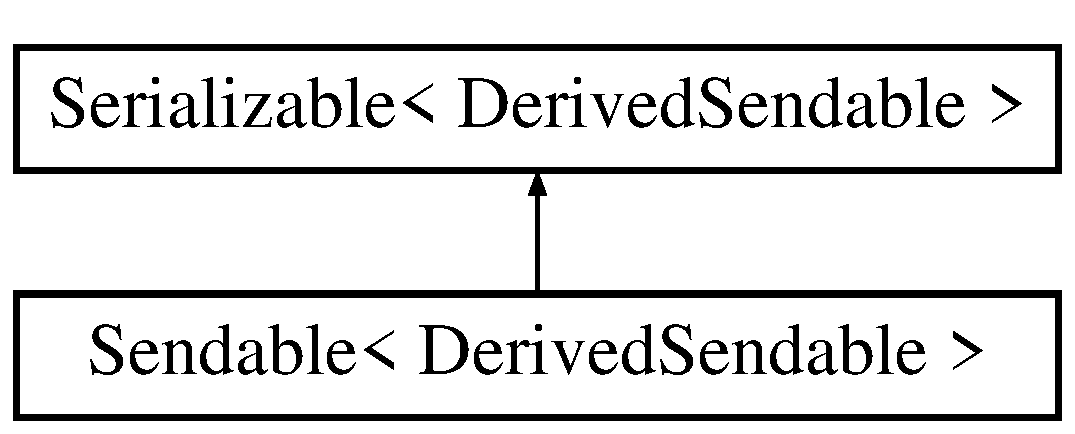
\includegraphics[height=2.000000cm]{classSendable}
\end{center}
\end{figure}
\subsection*{Public Member Functions}
\begin{DoxyCompactItemize}
\item 
{\footnotesize template$<$typename Recipient $>$ }\\void \hyperlink{classSendable_acd9845338560f7c51e5e6e57d282c127}{tb\-\_\-sendto} (Recipient receiver)
\item 
virtual int \hyperlink{classSendable_a8d13bbd5c89dc4dc2da25e8f344c550e}{get\-Sendable\-Type} ()=0
\end{DoxyCompactItemize}


\subsection{Detailed Description}
\subsubsection*{template$<$class Derived\-Sendable$>$class Sendable$<$ Derived\-Sendable $>$}

\hyperlink{classSendable}{Sendable} class which utilizes Curiously Recurring Template Pattern (C\-R\-T\-P) to get the \char`\"{}this\char`\"{} object of the derived class instead of itself.

It has only one public function, which is basically \char`\"{}\-I am transmitting myself to someone\char`\"{} function.

This class inherits \hyperlink{classSerializable}{Serializable} class which directly implements B\-O\-O\-S\-T\-::serialize library.


\begin{DoxyTemplParams}{Template Parameters}
{\em Derived\-Sendable} & derived class that inherits this \hyperlink{classSendable}{Sendable} class. \\
\hline
\end{DoxyTemplParams}


\subsection{Member Function Documentation}
\hypertarget{classSendable_a8d13bbd5c89dc4dc2da25e8f344c550e}{\index{Sendable@{Sendable}!get\-Sendable\-Type@{get\-Sendable\-Type}}
\index{get\-Sendable\-Type@{get\-Sendable\-Type}!Sendable@{Sendable}}
\subsubsection[{get\-Sendable\-Type}]{\setlength{\rightskip}{0pt plus 5cm}template$<$class Derived\-Sendable $>$ virtual int {\bf Sendable}$<$ Derived\-Sendable $>$\-::get\-Sendable\-Type (
\begin{DoxyParamCaption}
{}
\end{DoxyParamCaption}
)\hspace{0.3cm}{\ttfamily [pure virtual]}}}\label{classSendable_a8d13bbd5c89dc4dc2da25e8f344c550e}
pure virtual method that N\-E\-E\-D\-S T\-O B\-E O\-V\-E\-R\-R\-I\-D\-E\-N \begin{DoxyReturn}{Returns}
type of the \hyperlink{classSendable}{Sendable} based on Enum (T\-C\-P\-\_\-\-T\-Y\-P\-E\-\_\-\-L\-I\-S\-T) 
\end{DoxyReturn}
\hypertarget{classSendable_acd9845338560f7c51e5e6e57d282c127}{\index{Sendable@{Sendable}!tb\-\_\-sendto@{tb\-\_\-sendto}}
\index{tb\-\_\-sendto@{tb\-\_\-sendto}!Sendable@{Sendable}}
\subsubsection[{tb\-\_\-sendto}]{\setlength{\rightskip}{0pt plus 5cm}template$<$class Derived\-Sendable $>$ template$<$typename Recipient $>$ void {\bf Sendable}$<$ Derived\-Sendable $>$\-::tb\-\_\-sendto (
\begin{DoxyParamCaption}
\item[{Recipient}]{receiver}
\end{DoxyParamCaption}
)\hspace{0.3cm}{\ttfamily [inline]}}}\label{classSendable_acd9845338560f7c51e5e6e57d282c127}
The only public method of \hyperlink{classSendable}{Sendable} class.


\begin{DoxyTemplParams}{Template Parameters}
{\em Recipient} & Any class that inherits \hyperlink{classReceivable}{Receivable} class. \\
\hline
\end{DoxyTemplParams}

\begin{DoxyParams}{Parameters}
{\em receiver} & any \hyperlink{classReceivable}{Receivable} object \\
\hline
\end{DoxyParams}


The documentation for this class was generated from the following file\-:\begin{DoxyCompactItemize}
\item 
/home/hspark/\-Dev\-Works/\-H-\/\-Tmax/cpp\-Tests/\-Message\-Protocol/\-T\-C\-P/\hyperlink{Sendable_8h}{Sendable.\-h}\end{DoxyCompactItemize}

\hypertarget{classSerializable}{\section{Serializable$<$ Derived\-Serializable $>$ Class Template Reference}
\label{classSerializable}\index{Serializable$<$ Derived\-Serializable $>$@{Serializable$<$ Derived\-Serializable $>$}}
}
\subsection*{Public Member Functions}
\begin{DoxyCompactItemize}
\item 
std\-::string \hyperlink{classSerializable_a59ea122ccd8fc4c7d72d9a7e57a2ea0a}{marshal} ()
\item 
void \hyperlink{classSerializable_a802e37fd701dc56319d464a9ecc5fe07}{unmarshal} (std\-::string serialized)
\end{DoxyCompactItemize}
\subsection*{Friends}
\begin{DoxyCompactItemize}
\item 
class \hyperlink{classSerializable_ac98d07dd8f7b70e16ccb9a01abf56b9c}{boost\-::serialization\-::access}
\end{DoxyCompactItemize}


\subsection{Member Function Documentation}
\hypertarget{classSerializable_a59ea122ccd8fc4c7d72d9a7e57a2ea0a}{\index{Serializable@{Serializable}!marshal@{marshal}}
\index{marshal@{marshal}!Serializable@{Serializable}}
\subsubsection[{marshal}]{\setlength{\rightskip}{0pt plus 5cm}template$<$class Derived\-Serializable$>$ std\-::string {\bf Serializable}$<$ Derived\-Serializable $>$\-::marshal (
\begin{DoxyParamCaption}
{}
\end{DoxyParamCaption}
)\hspace{0.3cm}{\ttfamily [inline]}}}\label{classSerializable_a59ea122ccd8fc4c7d72d9a7e57a2ea0a}
Calling this-\/$>$marshal will serialize the object, then returns it in a string (byte $\ast$)

\begin{DoxyReturn}{Returns}
serialized \char`\"{}this\char`\"{} object in a form of a std\-::string 
\end{DoxyReturn}
\hypertarget{classSerializable_a802e37fd701dc56319d464a9ecc5fe07}{\index{Serializable@{Serializable}!unmarshal@{unmarshal}}
\index{unmarshal@{unmarshal}!Serializable@{Serializable}}
\subsubsection[{unmarshal}]{\setlength{\rightskip}{0pt plus 5cm}template$<$class Derived\-Serializable$>$ void {\bf Serializable}$<$ Derived\-Serializable $>$\-::unmarshal (
\begin{DoxyParamCaption}
\item[{std\-::string}]{serialized}
\end{DoxyParamCaption}
)\hspace{0.3cm}{\ttfamily [inline]}}}\label{classSerializable_a802e37fd701dc56319d464a9ecc5fe07}
this-\/$>$unmarshl will deserilize the string input (byte $\ast$) and populate the \char`\"{}this\char`\"{} object


\begin{DoxyParams}{Parameters}
{\em serialized} & serialized \char`\"{}this\char`\"{} object in a form of a std\-::string \\
\hline
\end{DoxyParams}


\subsection{Friends And Related Function Documentation}
\hypertarget{classSerializable_ac98d07dd8f7b70e16ccb9a01abf56b9c}{\index{Serializable@{Serializable}!boost\-::serialization\-::access@{boost\-::serialization\-::access}}
\index{boost\-::serialization\-::access@{boost\-::serialization\-::access}!Serializable@{Serializable}}
\subsubsection[{boost\-::serialization\-::access}]{\setlength{\rightskip}{0pt plus 5cm}template$<$class Derived\-Serializable$>$ friend class boost\-::serialization\-::access\hspace{0.3cm}{\ttfamily [friend]}}}\label{classSerializable_ac98d07dd8f7b70e16ccb9a01abf56b9c}
B\-O\-O\-S\-T R\-E\-Q\-U\-I\-R\-E\-D V\-A\-R\-I\-A\-B\-L\-E 

The documentation for this class was generated from the following file\-:\begin{DoxyCompactItemize}
\item 
/home/hspark/\-Dev\-Works/\-H-\/\-Tmax/cpp\-Tests/\-Message\-Protocol/\-T\-C\-P/\hyperlink{Serializable_8h}{Serializable.\-h}\end{DoxyCompactItemize}

\hypertarget{structTCPHeader}{\section{T\-C\-P\-Header Struct Reference}
\label{structTCPHeader}\index{T\-C\-P\-Header@{T\-C\-P\-Header}}
}
\subsection*{Public Attributes}
\begin{DoxyCompactItemize}
\item 
\hypertarget{structTCPHeader_a61c09fc896a293dcbbab75586b782221}{int {\bfseries sendable\-Type}}\label{structTCPHeader_a61c09fc896a293dcbbab75586b782221}

\item 
\hypertarget{structTCPHeader_a6bbddb1f01512ba4e20a462d520fc8c6}{int {\bfseries payload\-Size}}\label{structTCPHeader_a6bbddb1f01512ba4e20a462d520fc8c6}

\item 
\hypertarget{structTCPHeader_a7b984e1a1c433954f80a6a1a8221f096}{bool {\bfseries payload\-Split}}\label{structTCPHeader_a7b984e1a1c433954f80a6a1a8221f096}

\end{DoxyCompactItemize}


The documentation for this struct was generated from the following file\-:\begin{DoxyCompactItemize}
\item 
/home/hspark/\-Dev\-Works/\-H-\/\-Tmax/cpp\-Tests/\-Message\-Protocol/\-T\-C\-P/T\-C\-P.\-h\end{DoxyCompactItemize}

\chapter{File Documentation}
\hypertarget{Sendable_8h}{\section{/home/hspark/\-Dev\-Works/\-H-\/\-Tmax/cpp\-Tests/\-Message\-Protocol/\-T\-C\-P/\-Sendable.h File Reference}
\label{Sendable_8h}\index{/home/hspark/\-Dev\-Works/\-H-\/\-Tmax/cpp\-Tests/\-Message\-Protocol/\-T\-C\-P/\-Sendable.\-h@{/home/hspark/\-Dev\-Works/\-H-\/\-Tmax/cpp\-Tests/\-Message\-Protocol/\-T\-C\-P/\-Sendable.\-h}}
}


\hyperlink{classSendable}{Sendable} header file for T\-C\-P (Tibero Communication Protocol)  


{\ttfamily \#include \char`\"{}T\-C\-P.\-h\char`\"{}}\\*
\subsection*{Classes}
\begin{DoxyCompactItemize}
\item 
class \hyperlink{classSendable}{Sendable$<$ Derived\-Sendable $>$}
\end{DoxyCompactItemize}


\subsection{Detailed Description}
\hyperlink{classSendable}{Sendable} header file for T\-C\-P (Tibero Communication Protocol) \begin{DoxyAuthor}{Author}
hspark 
\end{DoxyAuthor}
\begin{DoxyDate}{Date}
2018-\/\-F\-E\-B-\/12 
\end{DoxyDate}
\begin{DoxyVersion}{Version}
1.\-0 Any class that inherits the \hyperlink{classSendable}{Sendable} class can use \char`\"{}tb\-\_\-sendto\char`\"{} function to send itself to another class that inherits Recievable class. 
\end{DoxyVersion}

\hypertarget{Serializable_8h}{\section{/home/hspark/\-Dev\-Works/\-H-\/\-Tmax/cpp\-Tests/\-Message\-Protocol/\-T\-C\-P/\-Serializable.h File Reference}
\label{Serializable_8h}\index{/home/hspark/\-Dev\-Works/\-H-\/\-Tmax/cpp\-Tests/\-Message\-Protocol/\-T\-C\-P/\-Serializable.\-h@{/home/hspark/\-Dev\-Works/\-H-\/\-Tmax/cpp\-Tests/\-Message\-Protocol/\-T\-C\-P/\-Serializable.\-h}}
}


\hyperlink{classSerializable}{Serializable} header file.  


{\ttfamily \#include $<$boost/archive/binary\-\_\-oarchive.\-hpp$>$}\\*
{\ttfamily \#include $<$boost/archive/binary\-\_\-iarchive.\-hpp$>$}\\*
{\ttfamily \#include $<$boost/serialization/vector.\-hpp$>$}\\*
{\ttfamily \#include $<$sstream$>$}\\*
\subsection*{Classes}
\begin{DoxyCompactItemize}
\item 
class \hyperlink{classSerializable}{Serializable$<$ Derived\-Serializable $>$}
\end{DoxyCompactItemize}


\subsection{Detailed Description}
\hyperlink{classSerializable}{Serializable} header file. \begin{DoxyAuthor}{Author}
hspark 
\end{DoxyAuthor}
\begin{DoxyDate}{Date}
2018-\/\-F\-E\-B-\/12 
\end{DoxyDate}
\begin{DoxyVersion}{Version}
1.\-0 Any class that inherits the \hyperlink{classSerializable}{Serializable} class can serialize \& deserialize itself. Courtesy of B\-O\-O\-S\-T\-::serialization library 
\end{DoxyVersion}

%--- End generated contents ---

% Index
\newpage
\phantomsection
\addcontentsline{toc}{chapter}{Index}
\printindex

\end{document}
